
\chapter{Intrusion Detection Systems} \label{chap:Intrusion Detection Systems}


\section*{Introduction}
With the birth of the smart grid as the next step of evolution for grid infrastructure, with the improvements that the smart grid came with, like improved reliability, automation, and faster detection and response to failures, it also came with its own set of risks and disadvantages. mainly due to the fact that it is composed of multiple components and systems that are connected to the internet, like wireless networks and sensors, smart meters, and IoT devices, making it an easy target for hackers. independent groups or state actors whose goal is to cause as much damage as possible or to collect valuable data. On top of those components, there are legacy systems that the smart grid relies on that are known for their many and major security vulnerabilities, which are all easy targets, for example, Supervisory Control and Data Acquisition (SCADA). As an example of those risks and weaknesses, we can look at the situation Ukraine found itself in after Russia targeted their smart grid systems in 2015, leaving 80,000 Ukrainian households without power for 3 to 6 hours. \cite{ukrain-sg-attack}.

That's why it is important to protect the smart grid system from cyberattacks by employing IDS, IPS, and IDPS. 
as the second line of defense in case encryption and authorization were unsuccessful in stopping the cyberattack from targeting the smart grid system.

\newpage




\section{Intrusion detection systems (IDS)}
An intrusion detection system is a piece of hardware or software that is responsible for detecting suspicious and malicious activity, and in a network or an information system, the anomaly can either be reported to a systems administrator or saved to a security information and even management system (SIEM), the SIEM combines the output from multiple sources, then uses some filtering techniques to decide if the reported activity is malicious. \cite{ids-def}
An IDS on its own cannot stop intrusions; it can only detect and report them. However, with its evolution, the intrusion prevention system (IPS) or intrusion detection and prevention system (IDPS) can counter an attack. \cite{ibm-ids}








\section{Intrusion detection systems architecture}
Intrusion detection systems, like any complex system, are made of multiple interoperating components with a specific task assigned to each component. Although the functioning of an IDS changes vastly between different types of IDSs (different in deployment or detection methods), they all share a common general architecture, which is composed of the following components as shown in Figure \ref{fig:arch_IDS} \cite{arch-IDS}:

\begin{figure}[h]
	\centering
	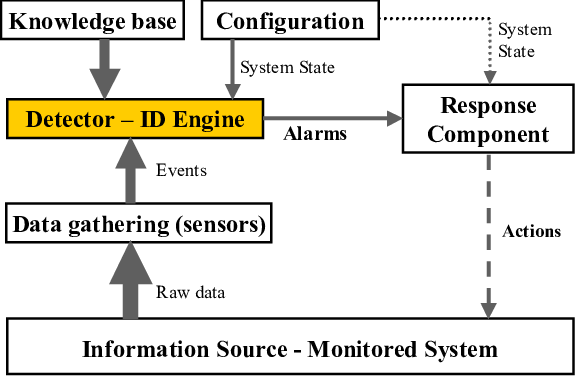
\includegraphics[width=400px]{figures/arch_IDS.png}
	\caption{IDS architecture \cite{arch-IDS}}
	\label{fig:arch_IDS}
\end{figure}

\firmlist
\begin{itemize}
	\item Data gathering components (sensor): tasked with collecting information from the monitored environment.
	\item Detector (IDS engine): analyzes the data collected by the sensor to determine the presence of suspicious activity.
	\item Knowledge base(database): the database that stores information collected previously by sensors about known attacks that allows the engine to determine the suspesious activity.
	\item Configuration component: defines settings and the behaviour of the system.
	\item Response component: this component is responsible for responding to the detected intrusion and either attempts to prevent the intrusion (IPS) or reports it to a human administrator (IDS).
\end{itemize}



\section{Intrusion detection systems classification}
Intrusion detection systems are classified according to two criteria of classification, which as shown in Figure \ref{fig:IDS-classification-taxonomy} are:

\firmlist
\begin{itemize}
	\item deployment method \cite{ids-classification}
	\item detection method \cite{ids-classification}
\end{itemize}




\begin{figure}[h]
	\centering
	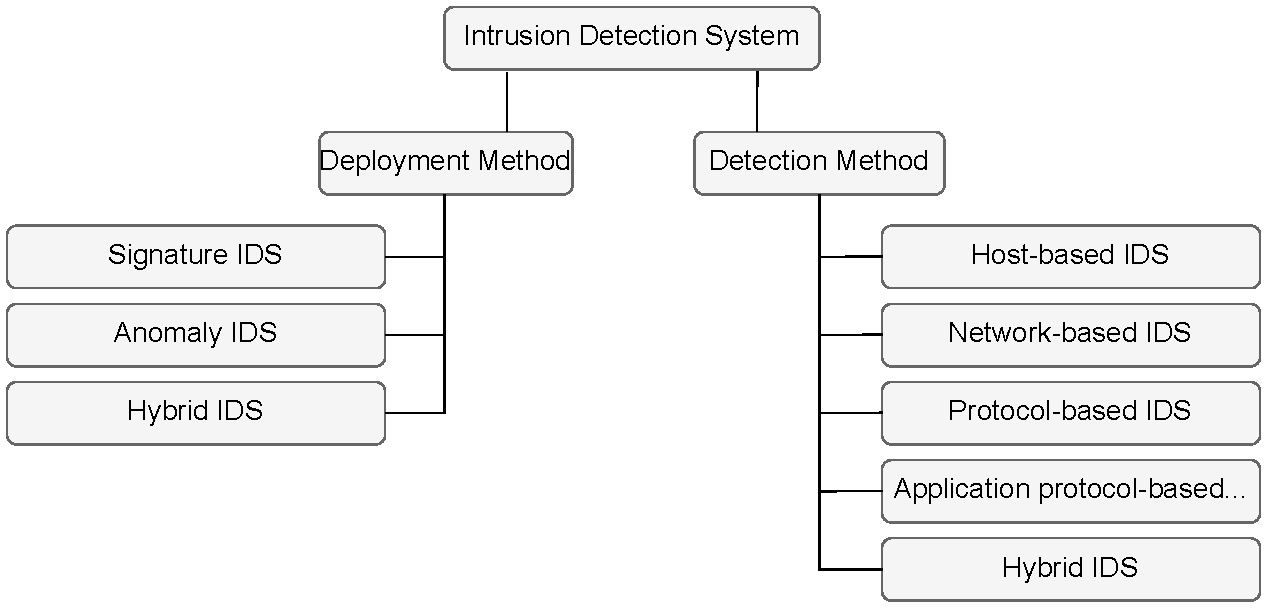
\includegraphics[width=400px]{figures/IDS_classification.pdf}
	\caption{IDS classification taxonomy}
	\label{fig:IDS-classification-taxonomy}
\end{figure}



\subsection{Deployment methods}
The deployment of IDS involves several methods that ensure effective monitoring and detection of potential threats. Here are some common deployment methods for IDS.

\subsubsection{NIDS}
Network intrusion detection systems are the most commonly used commercial IDS. They are usually placed at the start edge of the sub-network, right after the firewall (if one exists), so they can have access to all inbound traffic to all devices on the network \cite{NIST-IDS}. NIDS protects the networks from cyber attacks and threats by scanning and monitoring TCP/IP packets for known attack signatures and reporting them to the administrator \cite{NIDS-ip-tcp}

Some benefits of using a NIDS are that a few well-placed NIDS can be enough to cover an entire large network. In addition, their deployment requires minimal refactoring of the network, meaning easy installation \cite{NIST-IDS}. But the downsides are that they cannot detect threats with inaccurately constructed attack signatures and cannot analyze encrypted traffic, and it is hard to work with networks operating at 10 Gbps \cite{NIDS-ip-tcp}.

With a NIDS, one would ideally scan all inbound and outbound traffic; however, doing so might create a bottleneck that would impair the overall speed of the network.


\begin{figure}[h]
	\centering
	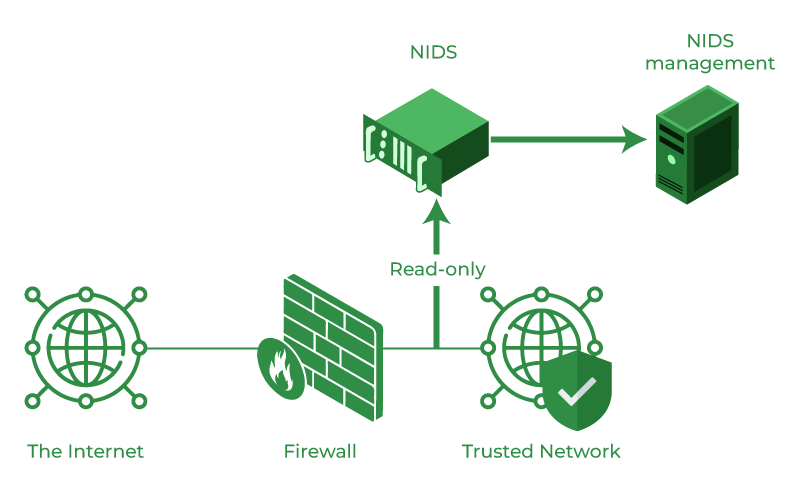
\includegraphics[width=300px]{figures/NIDS.png}
	\caption{NIDS \cite{geeksforgeeks}}
	\label{fig:NIDS}
\end{figure}



\subsubsection{HIDS}
Unlike NIDS, HIDS run on individual devices in a network, making it's threat detection scope more focused. They monitor all incoming and outgoing traffic and alert the administrator if suspicious or malicious activity is detected.

It is considered to be more reliable than NIDS because it has access to files in the operating system, and it can detect if a file has been tampered with by keeping snapshots of previous versions of those system files and comparing them to the current version to decide if it has been tampered with. \cite{NIST-IDS}

This type of IDS uses 2 sources of information inside the device's operating system:

\firmlist
\begin{itemize}
	\item system audit trails: operating system audit trails are created by the kernel making them very detailed because the kernel has access to everything in an OS. \cite{NIST-IDS}
	\item system logs: less complex the system audit trails making them easier to understand. \cite{NIST-IDS}
\end{itemize}



\begin{figure}[h]
	\centering
	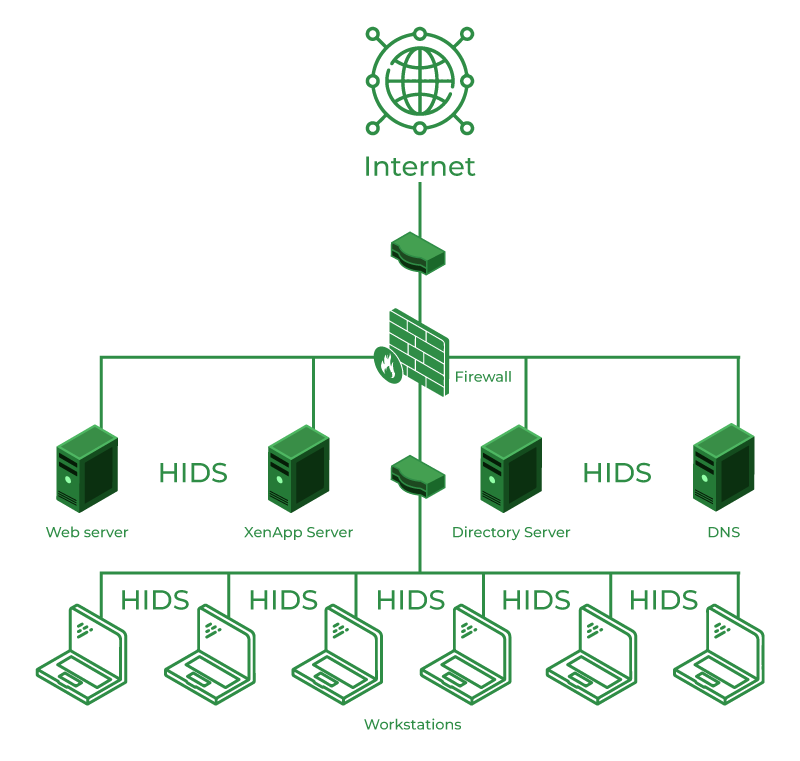
\includegraphics[width=300px]{figures/HIDS.png}
	\caption{HIDS \cite{geeksforgeeks}}
	\label{fig:HIDS}
\end{figure}



\subsubsection{Other types of IDS}
uncommon types with specific functions usually, used together with NIDS or HIDS to augment their detection capabilities.

\firmlist
\begin{itemize}
	\item Protocol intrusion detection system (PIDS): this type of IDS monitors the protocol in use (like HTTP or HTTPS) between the server and the client. PIDS is usually placed at the front end of the server. \cite{geeksforgeeks}


	\item Application protocol detection system (APIDS): specialized in application security, it analyzes the packets of application-specific protocols (like MySQL) to determine the presence of suspicious activity. APIDS are usually placed on groups of servers. \cite{geeksforgeeks}
	

	\item hybrid detection system: it is a combination of two or more of any of the previously defined IDSs. It is more reliable than any individual IDS because it has access to the data accessible to all of the used IDSs, providing it with a network-wide view.
	\cite{geeksforgeeks}
\end{itemize}




\subsection{Detection methods}
There are two primary methodes of detection for IDS which are anomaly-based and signature-based (which is also known as misuse intrusion detection or knowledge-based intrusion detection). \cite{ids-classification}



\subsubsection{Signature-based detection}
SIDs define patterns in known cyberattacks and store them in a database as signatures. The SID then analyzes system activity and search for a pattern of suspicious activity that matches previously documented attacks's signatures. This method provides high detection capabilities against known attacks. even though it cannot detect new attacks. On top of that, the database of previous attacks is very large, and having to compare internet packets to this database is resource- and time-consuming. \cite{NIST-IDS}



\subsubsection{Anomaly-based detection}
AIDs can identify abnormal behaviour in the environment it is used in, this type of IDS first observes and models the normal behaviours then compares the trffic to this model to determine the presnece of suspesious activity. the constructed model is created based on the data collected by observing the behaviour of the system over a specific period of time of normal operation. \cite{NIST-IDS}

AIDs often lead to a lot of false negatives because the normal activity varies alot over time, althout it is better than SIDs in detecting new and unknown attacks. it can also be used to provide new data for the signature-based detection systems. \cite{NIST-IDS}




\subsubsection{Hybrid detection}
Hybrid IDS uses both Signature based and anomaly based detection althout it's not widely used because it is still in development. \cite{NIDS-ip-tcp}
\clearpage

\subsubsection{Signature-based VS Anomaly-based detection}
table of pros and cons
sigVSano.tex
\begin{table}[h]
	\centering
	\caption{An example of tables}
	\begin{tabular}{|L{1.2cm}C{7cm}R{7cm}|}  % sum=15.2cm (L=Left, C=Center, R=Right)
	\hline
	& Signature-based & Anomaly-based \\
	Pros &
	\firmlist
	\begin{itemize}
		\item simple and effective against know attacks
		\item fewer false positives
	\end{itemize}
	&
	\firmlist
	\begin{itemize}
		\item Ineffecitve againts new and unknown attacks
		\item slow if the database is large
		\item database needs to be cosntantly constanlty maintained and updated
	\end{itemize}
	\\

	Cons &
	\firmlist
	\begin{itemize}
		\item can detect new and unknown attacks
		\item can provide data to Signature-based detection
	\end{itemize}
	&
	\firmlist
	\begin{itemize}
		\item more false negatives
		\item needs training to build normal behaviour models
	\end{itemize}
	\\
	\hline
\end{tabular}
	\label{tab:example}
\end{table}


The biggest disadvantage of an IDS is its inability to react to attacks and actively block malicious activity. That's why it was necessary to create a new system to overcome those drawbacks, which is IDPS, also known as IDPS, IDPS just like IDS monitors the activity of a network or a host scanning for attacks or malicious acitvity, the difference between them is that IDPS can actively block and prevent intrusions which it detects, IDPS can drop malicious internet packets, block traffic from a certain IP address or to a certain host, server, application or any targeted resource, it can also detect reconnaissance activity like port and host scans which indecates a potential future attack.

\section{Evolutions of IDS: IPS/IDPS}
The main drawback of an IDS is its inability to perform a response for the attack and actively prevent malicious activity. Because of that, a new system was developed to remove those vulnerabilities, and called IDPS, even though IDPS is similar to IDS when monitoring the network or host for the presence of attacks or malicious activity, it is different from IDS as it can be used to prevent such intrusion automatically, for example it can drop malicious packets from the internet, block or ban the IP address or the suspected traffic to the host, server or application, etc, Additionally, it is also able to recognise reconnaissance, such as port and host scans, which would suggest a future possible attack. \cite{NIST-IDPS}



\section{IPS/IDPS classification}
Just like IDS, IDPS is classified based on two criteria, including their deployment and detection methods as shown in Figure \ref{fig:IDPS-classification-taxonomy} are:

\begin{figure}[h]
	\centering
	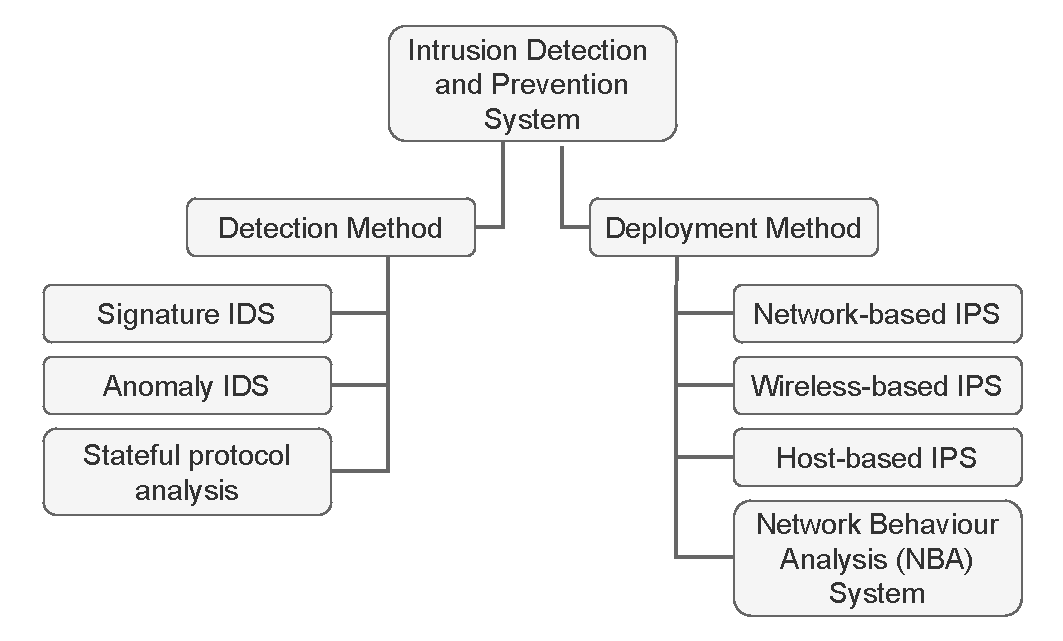
\includegraphics[width=400px]{figures/IDPS_classification.pdf}
	\caption{IDPS classification taxonomy}
	\label{fig:IDPS-classification-taxonomy}
\end{figure}




\subsection{Deployment methods}
\subsubsection{Network-based Prevention System (NIPS)}
A network-based prevention system (NIPS) is a network-based intrusion prevention system. It checks all internet packets inbound and outbound in a network, making it possible to detect suspicious activity. these monitoring devices are placed at a strategic point right at the start of a sub-network, usually being right behind the firewall. NIPS might also be placed within the network to watch over movement of data from important assets such as critical data centers or any other device. \cite{IBM-IPS}

\subsubsection{Wireless-based Prevention System (WIPS)}
A wireless intrusion prevention system (WIPS) is designed to monitor wireless network protocols for any signs of suspicious activity, like unauthorized users or devices connected to the the wifi in question. Once a WIPS notices that an unknown entity has connected to a wireless network, it can automatically cut the connection. A WIPS can also be utilized to recognize misconfigured and unsecure devices operating on a wifi network, and set up even to intercept man-in-the-middle attacks.\cite{IBM-IPS}

\subsubsection{Host-based Prevention System (HIPS)}
A host-based intrusion prevention system (HIPS) is installed in a particular device such as a laptop or server and monitors only the traffic that comes and goes through it. HIPS are commonly paired up with NIPS to provide additional protection for critical assets. In addition, HIPS can stop malware from moving between devices on the same network, as may happen when ransomware is unleashed.\cite{IBM-IPS}

\subsubsection{Network Behaviour Analysis (NBA) System}
A network behavior analysis (NBA) is a type of IPS that monitors the packets of a network, but unlike other types of IPS, this one focuses on high-level details like source/distonation IP addresses, ports, and the number of packets transmitted by those IP addresses. It uses an anomaly-based detection method that is effective in detecting and blocking abnormal behavior like DDoS attacks and communications with malware-infected devices.\cite{IBM-IPS}


\subsection{detection methods}

detection methods are the same in IPS as in IDS with stateful protocol analysis beign exclusive to IDPS, IDPS usually uses multiple detection methodes at the same time to broaden it's detection rates. \cite{NIST-IDPS}

IDPS has 3 primary detection methodes:


\begin{itemize}
	\item Signature-based: Signature based detection is fairly similar to that of IDS with the difference beign that IDPS is capable of blocking or countring the detected intrusion
	\item Anomaly-based: the same thing applies to Anomaly-based detection as the detection phase is the same between IDS and IDPS
	\item Stateful protocol analysis applies the technique of comparing observed user behavior with predefined profiles that define what is regarded as normal activity. What sets it apart from anomaly-based detection is that stateful protocol analysis employs vendor-specific profiles which define normal behavior of a protocol. In this type of IPS, network, transport, and application layer protocol states will be tracked in order for the Intrusion Detection Prevention System (IDPS) to understand the state transitions. Consequently, when a user logs into an FTP session in an unauthenticated state, he can only execute basic commands such as viewing help information or providing login credentials. As a result, this allows the Intrusion Detection and Prevention System to differentiate between suspicious and benign actions by checking whether they conform to what is expected at that particular point or not after pair requests with responses and successfully authenticating. \cite{NIST-IDPS19-20}
	

\end{itemize}









%###############################################################
%###############################################################
%###############################################################
%################################################# to be changed
%###############################################################
%###############################################################
%###############################################################
%\section{Cyberattacks on smart grid and their classification}
%the Smart grid is suseptibale to a wide variety of cyberattacks like malicious code, jamming, spoofing, injections, traffic eavesdropping, and social engineering just to name a few
%
%on this project we will be looking at some of the most commonly used attacks
%
%%https://arxiv.org/pdf/2207.07738 page 13
%%https://www.perplexity.ai/search/types-of-IDSP-xp9WyS2RTnihkZchcIzv_g
%
%
%\subsection{cyberattack types}
%\subsubsection{Denial-of-service attack}
%A denial-of-service attack is an attack in which the perpetrator sends a large amount of traffic to the target to overload it and render a service or a server incapable of processing legitimate user requests. \cite{dos}, some types of denial of service attacks are:
%\begin{itemize}
%	\item SYN flood: This happens when the attacker sends a 3-way handshake request without completing it, leaving the server waiting for a response and wasting time and resources that could be used by a legitimate user. \cite{dos}
%	\item smurf attack: the attacker sends ICMP (Internet Control Message Protocol) broadcast packets to some hosts in the network with a spoofed source IP address that is the IP of the target, those hosts would then respond to the spoofed IP address, flooding the target with those responses. This usually happens because of a misconfiguration of the devices on the network. \cite{dos}
%\end{itemize}
%
%Another version of DoS attacks is the distributed denial-of-service attack (DDoS), and what sets it apart from a normal DoS attack is the number of devices used in attack. DDoS usually leverages the use of botnets, which are infected machines controlled by the attacker. Having more devices means the ability to send an even larger amount of traffic to the target and also makes it harder to identify the attacker. \cite{dos}
%	
%
%\subsubsection{Malicious software}
%Malware, which stands for malicious software, is a computer- and user-harming program that steals information, corrupts files, or disrupts computers. Its wide presence greatly threatens the security of computers, thus hindering network growth and targeting network-based applications. Malware makers keep upgrading their tactics to avoid being detected by using encryption and morphing techniques such as polymorphism and metamorphism. Signature-based detection methods work well with known malware but struggle with new ones, especially those that are polymorphic. On the other hand, heuristic-based detection usually gives false negatives and positives despite its ability to identify both new and existing malicious programs. Therefore, machine-learning algorithms combined with data-mining techniques are incorporated into existing approaches for fighting against ever-changing malware threats in order to enhance the accuracy of detection. \cite{malware} Malware has multiple types. some of which are:
%
%	\begin{itemize}
%	\item Viruses: Viruses need a host program or file to infect and propagate in a system. They remain dormant until the host is executed; then, they insert their code into other programs, copy themselves, damage files and spread to more devices. Viruses depend on human interaction for their activation and spreading from one computer to another. some of the consequences of this type of malware are performance issues, data or money loss, privacy invasion, and large-scale and nation-state attacks. \cite{virusVSworm}
%	\item Worms: Worms are independent programs which do not require any hosts. They can reproduce themselves and propagate automatically in a system without being activated by humans leading them to spread very fast often throughout a local network, sometimes at exponential rates. Security vulnerabilities may allow worms into a system without user's consent. Worms are generally considered more dangerous than viruses due to their ability to spread more quickly and without human interaction.\cite{virusVSworm}
%	\item Trojans: A trojan horse usually appears as a harmless piece of software, once it is installed on a system it is a  dangerous malware. This malicious application often disguises as a legitimate file in email attachments or free software, waiting for the user to download them or click on them. Once infiltrated, the Trojan can carry out multiple functions as coded by it's author. The infection occurs after a user downloads a file containing the server side of the malicious software, which is then set up once it has been downloaded, the attacker spams emails to a lot of users with a torjan horse attached for download hoping those users will download it. Infected systems can infect other devices, forming a botnet.\cite{torjanhorse}
%	\end{itemize}
%
%Another type of Malware is Exploit kits which is used by cyber criminals to identify vulnerabilities in software or an operating system, then upload malicious code and execute it on their device. Those kits automatically exploit software vulnerabilities, often because the software is outdated. They work by redirecting the victim to compromised websites to identify vulnerabilities in their system and decides which exploits to use and uploading it to the user. If it succeeds, it downloads and executes a malicious piece of code that gives the attacker access to the victim's machine. \cite{exploit-kit}
%
%\subsubsection{injection attacks}
%code injection attacks is when a cyber criminal is capable of editing
%%need to complete
%
%\subsubsection{replay of messages}
%The replay attack takes place when a cyber criminal intercepts and forwards a secure network communication messages to deceive the recipient into doing something he is not allowed to do. reply of messages is very dangerous because no advanced decryption techniques are needed, only resending of the intercepted message, a captured message that is resent can be successful in this attack since it appears genuine due to its original encryption. One instance in real life involves a staff member who sends an encrypted message to the financial administrator requesting for a transfer of money. This message is intercepted, copied and then sent again by an attacker.The financial administrator sees that the request is properly encrypted hence would respond appropriately unless suspiciousness occurs. Consequently, this could lead to remitting of huge amount of money into the account of the hacker. \cite{replay}
%
%###############################################################
%###############################################################
%###############################################################
%################################################# to be changed
%###############################################################
%###############################################################
%###############################################################



%################################################# maybe to be changed
%\section{IDPS usage in smart grid}
%required to be able to do :
%
%\firmlist
%\begin{itemize}
%	\item detecting wide range of intrusions
%	\item fast detection
%	\item accuracy (FP/FN/TP/TN)
%	\item resource efficient
%	\item scalable
%	\item easy to operate (user friendly)
%\end{itemize}
%################################################# maybe to be changed





\section{Machine learning based intrusion detection system}
\subsection{A general AI-based NIDS methodology}






\section{conclusion}





